% requires \usepackage{pgfplots} and \pgfplotsset{compat=1.18} in the preamble
\definecolor{armNone}{HTML}{2A78D6}
\definecolor{armSumm}{HTML}{EB6834}
\definecolor{armAcm}{HTML}{1BAF7A}
\begin{figure}[t]
\centering
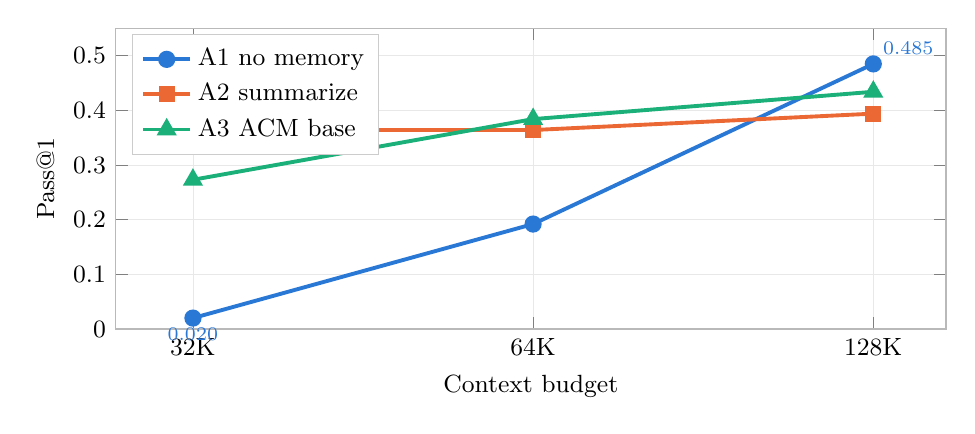
\begin{tikzpicture}
\begin{axis}[
  width=\columnwidth, height=5.4cm,
  xmode=log, log basis x=2,
  xtick={32768,65536,131072}, xticklabels={32K,64K,128K},
  xlabel={Context budget}, ylabel={Pass@1},
  ymin=0, ymax=0.55, ytick={0,0.1,0.2,0.3,0.4,0.5},
  xmin=28000, xmax=152000,
  grid=major, grid style={gray!18, line width=0.3pt},
  axis line style={gray!55, line width=0.5pt},
  tick label style={font=\small}, label style={font=\small},
  legend style={font=\small, draw=gray!40, fill=white, at={(0.02,0.98)},
                anchor=north west, row sep=1pt, inner sep=3pt},
  legend cell align=left,
  clip=false,
]
\addplot[armNone, line width=1.4pt, mark=*, mark size=2.4pt]
  coordinates {(32768,0.020) (65536,0.192) (131072,0.485)};
\addlegendentry{A1 no memory}
\addplot[armSumm, line width=1.4pt, mark=square*, mark size=2.2pt]
  coordinates {(32768,0.364) (65536,0.364) (131072,0.394)};
\addlegendentry{A2 summarize}
\addplot[armAcm, line width=1.4pt, mark=triangle*, mark size=2.8pt]
  coordinates {(32768,0.273) (65536,0.384) (131072,0.434)};
\addlegendentry{A3 ACM base}
% direct labels at the two ends, where the story is
\node[armNone, font=\scriptsize, anchor=north] at (axis cs:32768,0.020) {0.020};
\node[armNone, font=\scriptsize, anchor=south west] at (axis cs:131072,0.485) {0.485};
\node[armSumm, font=\scriptsize, anchor=south] at (axis cs:32768,0.364) {0.364};
\end{axis}
\end{tikzpicture}
\caption{Resolve rate against context budget for Qwen3.5-9B on 99 SWE-Bench
Verified instances. The value of context management is monotone in how tight the
budget is and changes sign: at 32K the baseline resolves 2 of 99 while memory
resolves 27 to 36, at 128K the baseline overtakes both. ACM report a single
operating point at 128K, where their measured gap is $+0.019$.}
\label{fig:cap-sweep}
\end{figure}
